\documentclass[fontsize=12pt, paper=a4, headinclude, twoside=false, parskip=half+, pagesize=auto, numbers=noenddot, open=right, toc=listof, toc=bibliography]{scrreprt}
\usepackage[left=3cm, bottom=3cm, top=3cm]{geometry} % wenn es nicht anders geht sonst typearea (unten)
\usepackage{multirow} % Tabellen-Zellen über mehrere Zeilen
\usepackage{multicol} % mehre Spalten auf eine Seite
\usepackage{tabularx} % Für Tabellen mit vorgegeben Größen
\usepackage[automark]{scrpage2} % Kopf- und Fußzeilen
\usepackage[T1]{fontenc} % Ligaturen, richtige Umlaute im PDF 
\usepackage[utf8]{inputenc}% UTF8-Kodierung für Umlaute usw
\usepackage{bibgerm} % Bibliographie Umlaute in BibTeX
\usepackage{mathtools}

 
 \newcommand{\ourtitlepage}{
 %++++++++++++++++++++++++++++++++++++++++++++++++++++++++++++++++++
% Titelseite
%\clearscrheadings\clearscrplain
\begin{center}
{\large Universität Leipzig}\\
{\large Fakultät für Mathematik und Informatik}\\
{\large Institut für Informatik}\\
{\large Abteilung Automatische Sprachverarbeitung}\\
\vspace{5cm}
\begin{Large}
\textbf{Wortschatz Zeitgeist}\\
\vspace{5mm}
Seminararbeit\\
\vspace{5mm}
\end{Large}
\vspace{9cm}
\begin{tabular}{ r l }
{\bf Autoren:} 	& Döring, Thomas\\
			& Kießling, Max\\
			& Otto, Wolfgang (2885214)\\
{\bf Modul:} & Anwendungen Linguistische Informatik (10-202-2307)\\
{\bf Abgabe:} & {\today}. (Sommersemester 2015)\\
{\bf Betreuer:} & Maciej Janicki\\
{\bf Seminarleiter:}&Prof. Dr. Uwe Quasthoff\\ 
\end{tabular}\\
\end{center}
\clearpage

}


\begin{document}
\ourtitlepage 
\tableofcontents
\pagenumbering{roman} % Inhaltsverzeichnis roemisch 
\clearpage
\pagenumbering{arabic} % ab jetzt die normale arabische Nummerierung



% EINLEITUNG ###################################################################################
\chapter{Einleitung}

%##########################################
\section{Aufgabenstellung}
Das Portal  \emph{Wörter des Tages}\footnote{\url{http://wortschatz.uni-leipzig.de/wort-des-tages}, Abgerufen am 29.10.2015,~9:34~Uhr} stellt eine Übersicht von Wörtern, die an einem ausgewählten Tag besonders relevant erschienen dar. Die Wörter sind in neun Kategorien eingeordnet. Nach der Beschreibung auf der Website werden die Wörter ermittelt in dem die tagesaktuelle Häufigkeit eines Wortes mit seiner durchschnittlichen Häufigkeit über längere Zeit hinweg gemessen wird.\\
Die Aufgabe dieser Arbeit ist es verschiedene Möglichkeiten der Bestimmung von Wörtern, die an einem gewählten Tag von besonderer Relevanz sind zu beschreiben, zu vergleichen und zu evaluieren. 
Die Datengrundlage zur Erstellung der Wörter des Tages ist ein Corpus, das durch tägliches crawlen von Newsseiten generiert wird. Die Quellen der Newseiten sind eine definierte Menge an für relevant erachtete Seiten mit Nachrichten wie zum Beispiel \emph{Spiegel.de}.\\
Bei allen Ansätzen, die auf das Vorkommen in einem Referenzzeitraum rekurrieren besteht das Korpus aus allen gecrawlten Newsseiten des voragngegangenen Jahres (2014).
Als Zusatzaufgabe soll ein musterbasiertes Verfahren in SQL entworfen werden, das es ermöglicht aufgrund eines gewählten Verfahrens falsch identifizierte Wörter zu filtern. Ein Beispiel hierfür sind Datumsangaben, die als relevant erscheinen, da sie Tagesaktuell oft auftauchen, aber im Vergleichszeitraum selten.

%##########################################
\section{Vergleichbare Ansätze}
Das Problem der Trenderkennung ist ein vielfältiges Problem mit einer großen Bandbreite an Anwendungsgebieten. Eine der vielleicht populärsten Anwendungen ist die Erkennung von Trendbegriffen bei Twitter, einem Microbloging-Dienst mehreren hundert Millionen Nutzern und 500 Mio Tweets täglich. Aufgrund dieser immensen Vielfalt an Nutzern und Nachrichten ist es möglich, dass hochaktuelle Nachrichten und Neuigkeiten rasend schnell global verbreitet werden können. Mithilfe von Trendanalyse ist es möglich globale aber auch lokale Entwicklungen zeitig zu erfassen und zu analysieren.
Einen ähnlichen Ansatz verfolgt das Google Projekt \emph{Google Trends}. Hier werden die Suchenanfragen der weltweit größten Websuchmaschine ausgewertet, wodurch die zeitabhängige Auswertung einzelner Suchbegriffe möglich wird. \\
Aber auch bei kleinerer Datenmengen ist das Erkennen von Trends bzw. Anomalien nützlich. Angewand auf Logdateien ist es so zum Beispiel möglich Angriffe auf ein Computersystem zu erkennen. \cite{Zwietasch14}


% HAUPTTEIL THEORIE ##########################################################################
%\chapter{Methoden zum Finden tagesaktueller Wörter}

%##########################################
\chapter{Maße zur Trend-Detection}
Im folgenden Abschnitt werden fünf Methoden vorgestellt, die f\"uer jedes Wort eines Tageskorpus eine Maßzahl bestimmen, die die Relevanz des Wortes an diesem Tag ausdrücken soll.

%#####################

\section{Relatives Vorkommen (Referenz)}
Ein einfacher Ansatz, der als Referenz zum Finden relevanter Wörter eines Tages dient ist der, das Auftreten jedes Tokens im Tageskorpus mit dem Auftreten im Referenzkorpus ins Verhältnis zu setzen.\\
Hierbei werden um eine Vergleichbarkeit zwischen verschiednen Tagen zu gewährleisten die Frequenzen der Wörter über die Anzahl aller Tokens im Tages bzw. Referenzkorpus normiert.\\

	\emph{Formel: } 
	\begin{equation}
	sig_{freqratio}(w) = \frac{\frac{k_{day}}{n_{day}}}{\frac{k_{2014}}{n_{2014}}}
	\end{equation}
	$k_{day}$: Frequenz des Tokens an einem Tag\\
	$n_{day}$: Summe der Frequenzen aller Tokens eines Tages\\
	$k_{2014}$: Frequenz des Tokens im Referenz Zeitrahmen (2014)\\
	$n_{day}$: Summe der Frequenzen aller Tokens im Referenzzeitraum (2014)\\
	

In Abbildung~\ref{pic.rel_freq} stellt die schwarze Gerade dar, wie sich der Wert der relativen Frequenz verhält, wenn die Anzahl des Auftretens eines Tokens variiert. Die senkrechte roten Linien markiert die Anzahl der Tokens, bei denen das relative Auftreten dem relativen Auftreten im Referenzkorpus entspricht. Der Wert der relativen Frequenz steigt also linear bei der Steigerung der Anzahl der Tokens eines Wortes.Dies führt zu der Problematik der Überschätzung von niederfrequenten Wörter im Referenzkorpus selbst bei relativ seltenem Auftreten im Tageskorpus. Bei niederfrequenten Wörtern ist der Anstieg der Gerade sehr viel steiler.\\
Um diesem Problem gerecht zu werden hilft es ein Maß für die Relevanz eines Wortes finden, welches ein geringe Überschreitung des relativen Anteils im Referenzkorpus weniger goutiert als eine höhere. Der Ansatz des Poisson Maß es (\ref{subsec.poisson}) versucht dem gerecht zu werden.\\
\begin{figure}[h!]
    \centering
    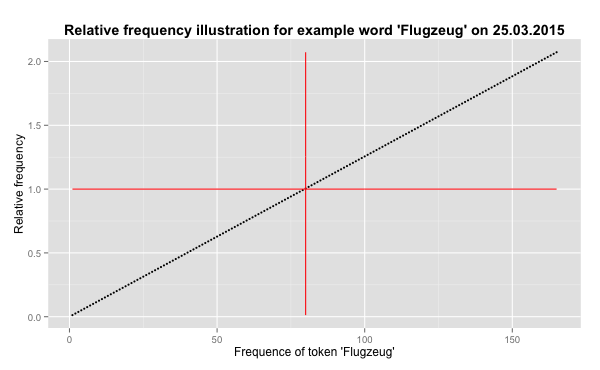
\includegraphics[width=1\textwidth]{pictures/relfreqFlugzeug.png}
    \caption{Illustration der relativen Frequenz des Tokens \enquote{Flugzeug} am 25.03.2015}\label{pic.rel_freq}
\end{figure}



\section{Poisson-Maß}\label{subsec.poisson}
Die Idee dieses Ansatzes ist es ein Maß zu nutzen, das die Wahrscheinlich Ausdrückt die gemessene Anzahl von Tokens eines Wortes an einem Tag zu beobachten. Auch hier wird zur Erstellung des Maßes  das Referenz

korpus des letzten Jahres genutzt. Die Annahme dieses Ansatzes ist nun, dass dieser Wahrscheinlichkeit die Poisson-Verteilung zugrundeliegt.\\
Die Formel~\ref{equ.poisson} ist die Poisson-Verteilung nach~\cite[S. 338 ff]{heyer06}.
	\begin{equation}\label{equ.poisson}
	P_\lambda(k) = \frac{\lambda^{k}}{k!}  \cdot e^{-\lambda}
	\end{equation}
	$\lambda$: Welche Frequenz wird erwartet \\
	(relativer Anteil im Referenzkorpus $\cdot$ Umfang des Tageskorpus)\\
	$k$: tatsächliches Auftreten von einem Wort k\\
	$P_\lambda(k)$: Erwartete Wahrscheinlichkeit meine Beobachtung k


In Abbildung~\ref{pic.poisson_algemein} ist exemplarisch die Wahrscheinlichkeit der Beobachtung der Token-Häufigkeit des Wortes Flugzeug abgebildet. Die Annahme besagt nun, dass je kleiner die Wahrscheinlichkeit
ist, desto relevanter erscheint ein Wort. \\

\begin{figure}[h!]
    \centering
    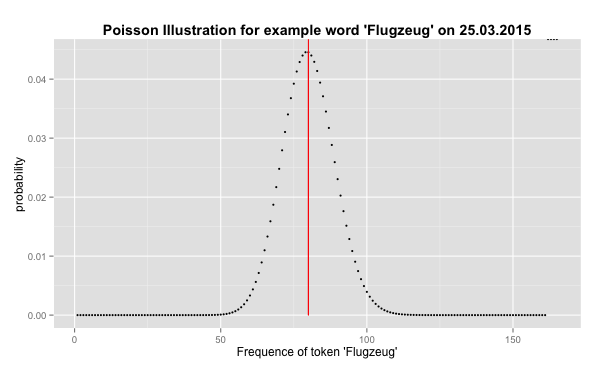
\includegraphics[width=1\textwidth]{pictures/poissonVerteilungFlugzeug.png}
    \caption{Illustration der Poissonverteilung des Token \enquote{Flugzeug} am 25.03.2015}\label{pic.poisson_algemein}
\end{figure}

An der Darstellung wird ein Nachteil dieser Methode deutlich. Nicht nur, wenn ein Token unerwartet oft beobachtet werden kann, auch wenn er seltener als erwartet beobachtet werden kann sinkt die Wahrscheinlichkeit nach diesem Modell beobachtet zu werden und es erscheint als relevantes Wort. Dieses Problem öst die im Folgenden beschriebene Transformation.\\

Ein weiteres Problem stellt der Rechenaufwand für diese Methode dar, da die Fakultät des tatsächlichen Auftretens $k$ eines Wortes berechnet werden muss. Die Herrleitung eines einfacher zu berechnenden 
equivalenten Maß es liefert~\cite[S. 338 ff]{heyer06}. Zu erwähnen ist, dass im Kontext dieser Herleitung wird das Maß allerdings nicht zur Bestimmung von in dieser Arbeit als relevant angesehenen Einzelwörtern genutzt. Sondern zur Bestimmung von signifikanten Kookurenzen. \\
Die Hergeleitete Formel~\ref{equ.poisson_mass} liefert drei Vorteile. Eine Berechnung der Fakultät ist nicht notwendig, die Anwendung des Logarithmus liefert ein positiven Wert für unwahrscheinliche Beobachtungen, wobei die differenzen gereade bei unwahrscheinlichen Beobachtungen stärker ins Gewicht fallen und yu letzt werden die Wahrschinlichkeiten für seltener als erwartete Tokenzahlen nicht berücksichtigt. 
 \begin{equation}\label{equ.poisson_mass}
		sig_{poisson}(w) = \frac{k(\log(k)-\log(n\cdot p) -1)}{\log(n)} 
 \end{equation}
k:= Anzahl der Token von w in Tagesbericht\\
n:= Anzahl der Tokens in Tagesbericht\\
p:= relativer Anteil eines Tokens am Jahreskorpus\\

Die Abbildung~\ref{pic.poisson_mass} illustriert die Entwicklung des Poissonmaß es bezogen auf die Variation des Vorkommens des Tokens Flugzeug. Hier wird sichtbar, dass die unterrepräsentetion keinen positiven Wert erzeugt und somit keinen Einfluss auf eine nach diesem Maß  geordnete Liste hat. In der Praxis sind genügend positive Werte dieses Maß es zu beobachten.\\
Die Formel~\ref{equ.poisson_mass} wurde im praktischen Teil dieser Arbeit genutzt.\\
 
% Hier Beispiel Flugzeug
\begin{figure}[h!]
    \centering
    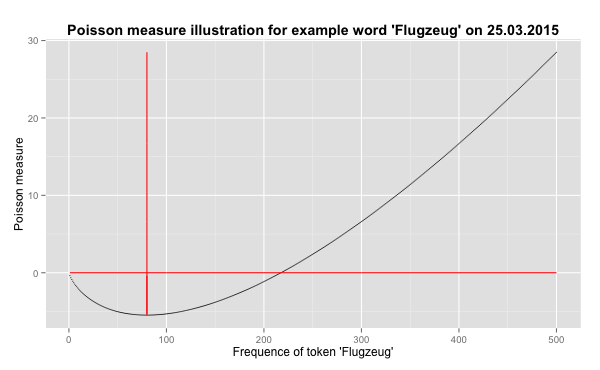
\includegraphics[width=1\textwidth]{pictures/poissonMeasureFlugzeug.png}
    \caption{Illustration des Poisson Maß es des Tokens \enquote{Flugzeug} am 25.03.2015}\label{pic.poisson_mass}
\end{figure}


\subsubsection{Bemerkungen zur Berechnung des Poisson-Maßes}
Die derzeitige Implementierung im Wortschatzporjekt der Universität Leipzig benutzt als Normierungsfaktor nicht die Anzahl aller Tokens im Tagesbericht. Auch zur Bestimmung des relativen Anteils eines Token am Jahreskorpus wird nicht die Anzahl der aller Tokens im Jahreskorpus, sondern die Anzahl der Sätze imJahreskorpus verwendet. Da bei der verwendeten Zahl von Sätzen das Verhältnis der Anzahl der Wörter zu der Anzahl der Sätze als konstant anzunehmen ist ($\approx 10$), scheint dies gerechtfertigt wie in~\ref{equ.word_sentence} formalisiert. 
\begin{equation}\label{equ.word_sentence}
\frac{|\text{Sätze}_{heute}|}{|\text{Sätze}_{jahr}|} \approx \frac{|Token_{heute}|}{|Token_{Jahr}|}
\end{equation}

Im Abschnitt~\ref{sec.quanitative_auswertung} wird diese Annahme durch einen Vergleich der sich ergebenden relevanten Wörter untersucht.

\section{Termfrequenz inverse Dokumentenfrequenz (tf-idf)}
Die Idee dieses Frequenzmaßes ist es, dass in der natürlichen Sprachverarbeitung breite Anwendung findende Maß TF/IDF für die Aufgabenstellung zu adaptieren. Dabei wird als Dokument das Korpus eines Tages im Referenzzeitraum betrachtet und für jedes Wort im Referenzzeitraum ein Wert bestimmt, der Angibt, an wie vielen Tagen das Wort im Jahr 2014 (Referenzzeitraum) aufgetreten ist. Verlgeiche dazu die Gleichung~\ref{equ.tfidf}.\\
\begin{equation}\label{equ.tfidf}
sig_{tf idf}(w) = \frac{k}{\max(K)} \cdot \log ( \frac{365}{|documentdays(w)|})
\end{equation}
$k$: Frequenz eines Tokens an einem Tag\\
$K$: Alle Frequenzen an einem Tag\\
Als Modifikation wird hier das gängige Verfahren der Logarithmisierung der inversen Dokumentfrequenz angewendet. Des weiteren wird, um eine Vergleichbarkeit über verschiedene Tage hinweg herrstellen zu könnnen, eine Relativierung der Frequenz auf Frequenz des häufigsten Tokens am Tag durchgeführt. Die graue Linie repräsentiert den idf-Wert, der zu der Entsprechung der relativen Tagesfrequenz führt, denn der Logarithmus von 2,7 ist ungefähr 1. Das entspricht dem Auftreten in ca. 8 Tagen des Referenzjahres.\\
% Hier Beispiel Flugzeug
\begin{figure}[h!]
    \centering
    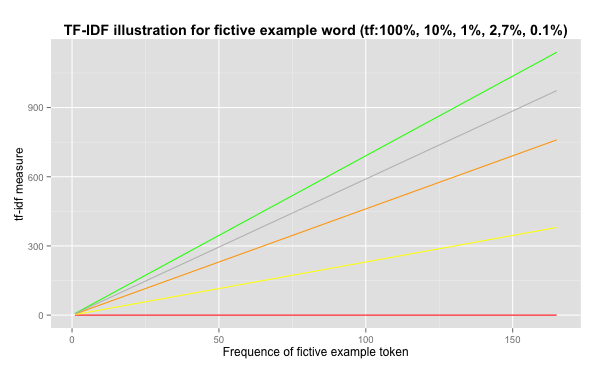
\includegraphics[width=1\textwidth]{pictures/tfidfIllustration.png}
    \caption{Illustration des TF/IDF Maßes anhand eines fiktiven Beispielworts}\label{pic.tfid_mass}
\end{figure}
Die Abbildung~\ref{pic.tfid_mass} verdeutlicht zwei Auswirkungen auf das Finden von relevanten Wörtern für die Aufgabenstellung. Zum einen ist das Grundlegende Problem, welches uns bei dem Maß des relativen Auftretens begegnete, dass niederfrequente Wörter überschätzt werden wieder vorhande, da mit steigender Frequenz die Maßzahl linear wächst. Allerdings wertet die inverse Dokumentenfrequenz häufige Wörter, wie Stoppwörter ab, was hilfreicht erscheint, da diese nicht als interessant zu bewerten sind.
Die rote Linie repräsentiert das Auftreten eines Worten an alle Tagen des Referenzkorpus. Die anderen Geraden bilden eine repräsentative Auswahl an weiteren Anteilen des Wortes an Tagen im Referenzjahr.\\

\section{Termfrequenz inverse Dokumentenfrequenz inverse Quellenfrequenz (tf-idf-isf)}
\emph{Idee: } Wörter sind dann interessant, wenn sie an einem Tag in möglichst vielen verschiedenen Quellen gennant werden.\\
Als Quelle definieren wir die Serveradresse einer Quelle. Diese wird mittels eines regulären Ausdrucks aus den zugeordneten Quellen in der MySQL-Datenbank ermittelt. Als Gesamtzahl der Quellen verwenden wir alle an einem Tag den Wörtern zugeordnete Quellen.\\
Das entstandene Signifikanzmaß wird in Gleichung~\ref{equ.tfidfsf} definiert.
\begin{equation}\label{equ.tfidfsf}
sig_{tf idf isf}(w) = sig_{tf idf}(w) \cdot \log ( \frac{Q_d}{q_d(w)})
\end{equation}
Analog zur inversen Dokumentenfrequenz wird also das tf-idf-Signifikanzmaß mit dem Logarithmus der inversen relativen Anzahl der Quellenfrequenz multipliziert. $Q_d$ ist die Anzahl aller erwähnten Quellen an einem Tag $d$ und $q_d()$ bildet ein Wort auf die Anzahl der Quellen ab, in denen das Wort an Tag $d$  erwähnt wird. 


%#####################
\subsection{Z-Score}
Benattar et al. beschreiben in \cite{benattar2011trend} einen Ansatz zur Trend-Erkennung basierend auf dem Z-Score. Dabei beziehen Sie neben der relativen Worthäufigkeit noch die Anzahl der Tage ein an denen ein Wort mindestens einmal auftritt, um so das 0-Frequenz-Problem zu umgehen.

\subsubsection{Berechnung}
\begin{itemize}
	\item{Wortfrequenz}\\
		$f(w)_d :=$ Anzahl der Vorkommen von Wort $w$ an Datum $d$
	\item{relative Worthäufigkeit}\\
		Die relative Worthäufigkeit $p(w)_d$ berechnet sich durch: \\
		$t_d :=$ Anzahl verschiedener Worte an Datum $d$
		$$ p(w)_d = \frac{f(w)_d}{t_d} \\ $$
	\item{Erwartungswert}\\
		Der Erwartungswert $\bar{w}$ berechnet sich durch: \\
		$N:=$ Anzahl der Tage in der betrachteten Zeitspanne
		$$\bar{w}=\frac{1}{N} \sum p(w)_d$$
	\item{Standartabweichung}\\
		Die Standartabweichung $\sigma_w$ berechnet sich durch:
		$$\sigma_w = \sqrt{\frac{1}{N} \sum (p(w)_d - \bar{w}^2}$$
	\item{ZScore}\\
		Der Zscore $Z(w)_d$ misst die Abweichung der relativen Worthäufigkeit vom Erwartungswert in Vielfachen der Standartabweichung.
		$$Z(w)_d= \frac{p(w)_d - \bar{w}}{\sigma_w}$$		
	\item{Auftrittshäufigkeit}\\
		Die Auftrittshäufigkeit $Po(w)$ gibt an wie vielen Tagen innerhalb des betrachteten Zeitraums das Wort mindestens einmal auftritt:\\
		$nbD(w) :=$ Anzahl der Tage an denen $w$ vorkommt//
		$c_d:=$ Anzahl der Tage innerhalb des betrachteten Zeitraums
		$$Po(w)=\frac{nbD(w}{c_d}$$
	\item{Schwellwerte}
		Zur besseren Unterscheidung echter Trends von statistischen Anomalien schlagen Benattar et. al. vor die Worte anhand ihrer Auftrittshäufigkeit zu clustern. Den Clustern werden dabei Z-Score-Schwellwerte zugeordnet. Überschreitet der Z-Score eines Wortes den Schwellwert seines Clusters wird dieses Wort als signifikant und somit als Trend eingestuft. Cluster mit niedriger Auftrittshäufigkeit erhalten dabei höhere Schwellwerte. Je häufiger ein Wort auftritt desto niedriger wird der Schwellwert. 
		
		
\end{itemize}

\subsubsection{Vorgehen}
\begin{enumerate}
	\item Für jedes Wort in $w$ in $d$ berechne $Z(w)$
	\item 
\end{enumerate}


%#####################
%\subsection{Weitere Maße}
%Einbeziehung der Anzahl von Quelle

%##########################################
\chapter{Zeitreihenanalysen}
Es wurde eine Pipeline in R geschrieben um geglättete Tagesfrequenzen zu berechnen.\footnote{Dieser Teil des Projektes wurde von Thomas Döring verfasst, der leider nicht in der Lage war bis Ende Oktober einen Beitrag zu dieser Arbeit zu leisten.} Diese Pipeline umfasst sechs Teile. Die Programmteile sind unter thomas/v2/R/1.r~-~6.r im Projektordner zu finden.
\begin{enumerate}
\item Aufbau einer Verbindung mit der Datenbank
\item Laden der Daten aus der Datenbank
\item Reshape der Daten I: Eine Spalte entspricht einem Wort
\item Berechnung der neuen Werte mittels Filter
\item Reshape der Daten II: Umformung in die Ursprüngliche Form mit einem Wort pro Zeile (melt)
\item Schreiben der berechneten Daten in die Datenbank 
\end{enumerate}
Die Abbildung~\ref{pic.time_airplane} stellt beispielhaft die Ergebnisse für das Wort Flugzeug dar. Mit der genutzten Bibliothek kann leicht durch Parameter die größe des Fensters angepasst werden.\footnote{Verwendete Funktion in R dokumentiert in: \url{https://stat.ethz.ch/R-manual/R-devel/library/stats/html/filter.html}, Abgerufen am 30.10.2015, 18:55 Uhr.}
% Hier Beispiel Flugzeug
\begin{figure}[h!]
    \centering
    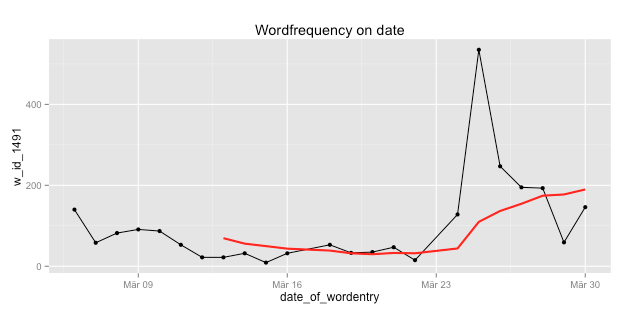
\includegraphics[width=0.82\textwidth]{pictures/timeFlugzeug.png}
    \caption{Illustration des gleitenden Fensters anhand des Wortes Flugzeug. Die rote Linie stellt die berechneten Werte dar. Die größe des Zeitfensters zur Durchschnittsbildung konnte leider nicht rekonstruiert werden (Annahme 8, da die ersten 7 Tage nicht geplottet sind). }\label{pic.time_airplane}
\end{figure}

 

%Cleanning ##########################################
\chapter{Cleaning}\label{cleaning}

Ein Problem welches alle im vorangegangen Kapitel vorgestellten Algorithmen gemein haben ist, dass Datumsangaben, sowie Uhrzeiten und Temperaturangaben häufig hohe Relevanzwerte erhalten. Vor allem die Datumsangaben des jeweiligen Tages werden täglich als Trend erkannt. Da diese jedoch keinen Informationswert besitzen sollten sie ausgefiltert werden. Der einfachste Ansatz ist diese Werte aus der Liste der Trends zu filtern. Dies kann mittels regulärer Ausdrücke realisiert werden. Die folgenden Ausdrücke können die häufigsten Vorkommen von Datums-, Zeit- und Temperaturangaben erkennen:

\begin{itemize}
	\item{Datumsangaben der Form 01.01, 01.01.15, 01.01.2015}\\
	\begin{lstlisting}[language=sql]
'^[[:digit:]]{2}.[[:digit:]]{2}(.[[:digit:]]{2,4})?$'
	\end{lstlisting}
\end{itemize}

\begin{itemize}
	\item{Datumsangaben der Form 01. Januar}\\
	\begin{lstlisting}[language=sql]
'^[[:digit:]]{2}.[[:blank:]](Januar|Februar|März|April|Mai|Juni|Juli|August|September|Oktober|November|Dezember)$'
	\end{lstlisting}
\end{itemize}

\begin{itemize}
	\item{Zeitangaben}\\
	\begin{lstlisting}[language=sql]
'[[:digit:]]{2}:[[:digit:]]{2}'
	\end{lstlisting}
\end{itemize}

\begin{itemize}
	\item{Temperaturangaben}\\
	\begin{lstlisting}[language=sql]
'[[:digit:]]{2}[[:blank:]]?°C?'
	\end{lstlisting}
\end{itemize}

Dieser Ansatz hat einen Nachteil, da alle Datumsangaben gefiltert werden. In einigen Ausnahmefällen könnten diese jedoch tatsächlich relevante Begriffe darstellen, als Beispiel sei hier der 11. September genannt. Da es sich bei den unerwünschten Angaben jedoch meist um das aktuelle Datum bzw. einen Tag später oder früher handelt, würde es ausreichen nur diese Ausdrücke zu filtern: 

\begin{itemize}
	\item{Datumsangaben gestern, heute, vorgestern}\\
	\begin{lstlisting}[language=sql]
SET lc_time_names = 'de_DE';
CONCAT("^(",
   CONCAT_WS("|",
       DATE_FORMAT(CURDATE(),"%d.%c.%Y"),
       DATE_FORMAT(CURDATE(),"%d.%c.%y"),
       DATE_FORMAT(CURDATE(),"%d.%c"),
       DATE_FORMAT(CURDATE(),"%d. %M"),
       DATE_FORMAT(CURDATE()-1,"%d.%c.%Y"),
       DATE_FORMAT(CURDATE()-1,"%d.%c.%y"),
       DATE_FORMAT(CURDATE()-1,"%d.%c"),
       DATE_FORMAT(CURDATE()-1,"%d. %M"),
       DATE_FORMAT(CURDATE()+1,"%d.%c.%Y"),
       DATE_FORMAT(CURDATE()+1,"%d.%c.%y"),
       DATE_FORMAT(CURDATE()+1,"%d.%c")
       DATE_FORMAT(CURDATE()+1,"%d. %M"),
   ),
   ")$"
);
	\end{lstlisting}
\end{itemize}



%HAUPTTEIL IMPLEMENTIERUNG ##################################################################
%\chapter{Implementierungen in SQL und R}



% AUSWERTUNG #################################################################################
\chapter{Ein empirischer Vergleich}

Die Messung der Güte der Ergebnisse stellt eine Herausforderung dar, da es keine geeignete Referenz, beispielsweise in Form eines Goldstandards der wichtigsten Worte eines Tages gibt. Um die Güte trotzdem einschätzen zu können bieten sich zwei Herangehensweisen an. Zum einen die eigenständige manuelle Prüfung der Ergebnisse unter selbst formulierten Kriterien, zum anderen der quantitative Vergleich mittels eines geeigneten Abstandsmaßes. Letzterer Ansatz bietet aber nur die Möglichkeit eines Vergleichs der Ähnlichkeiten der Ergebnisse und hilft abzuschätzen wie sich die Ergebnisse gegeneinander verhalten. Über die Güte gibt diese Methode keine Auskunft. Allerdings lassen sich Ausreißer gut erkennen und der Prämisse, dass gleiche Ergebnisse, die aus verschiedenen Messungen stammen eine höhere Wahrscheinlichkeit besitzen gute Ergebnisse zu sein lässt sich auch die Qualität beurteilen.
\section{Qualitativer Vergleich}
Aufgrund des fehlenden Goldstandards und Expertenwissen ist ein qualitativer Vergleich nur mittels Stichproben möglich. Jedoch ist selbst bei diesem Ansatz ein Bewertung der Ergebnisse schwierig. Wir haben uns daher entschieden den Vergleich an einem Tag durchzuführen und haben den 31.10.2015 ausgewählt. 
Für diesen Tag konnten wir daher zuerst mittels der Nachrichten eine Menge an Themen als Erwartungswert zusammenstellen. Wir erwarten daher, dass Begriffe welche diesem Thema zugeordnet werden können in den jeweiligen Listen vorkommen. Die Themen sind:
\begin{itemize}
	\item Flugzeugabsturz über dem Sinai
	\item Flüchtlingskrise
	\item Mordfall Elias und Mohamed
	\item Halloween
\end{itemize} 
Des weiteren sollte es möglich sein die anderen Trendworte aktuellen Themen zuordnen zu können, hierbei sollten überregionale Neuigkeiten vor Regionalen Themen priorisiert werden. 

\begin{table}
\centering
\resizebox{\textwidth}{!}{

\begin{tabular}{c|c|c|c}
\hline
Freqratio 							   & TF-IDF 					    & POISSON 						  & Z-Score \\
\hline

Zoo Leipzig               (129.6, 210) & Zoo Leipzig        (12,0, 210) & Zoo Leipzig         (69.3, 210) & Übergabe-          (7231.5,  10) \\
Flüchtlingskrise          (118.8, 124) & Gondwanaland       ( 8.2,  92) & Flüchtlinge         (67.9, 750) & Michls             ( 711.0,   8) \\
Gondwanaland              ( 94.7,  92) & Transitzonen       ( 7.6,  32) & Mohamed             (33.9, 172) & Ufo-Chef           ( 593.5,   7) \\
Transitzonen              ( 82.0,  32) & Flüchtlingskrise   ( 7.2, 124) & Gondwanaland        (32.1, 92 ) & Niedergörsdorf     ( 232.4,  16) \\
Lesbos                    ( 65.1,  62) & Graulich           ( 5.6,  42) & Zoo                 (31.6, 245) & Sachon             ( 217.3,   9) \\
lenkbare                  ( 61.9,  38) & Lesbos             ( 5.4,  62) & Mourinho            (29.2, 176) & 9268               ( 200.1,  12) \\
Hefei                     ( 51.1,  35) & Gräbersegnung      ( 4.6,  27) & Halloween           (22.9, 134) & Zoo Leipzig        ( 159.4, 210) \\
Elias                     ( 51.0, 187) & einDie             ( 4.5,  19) & Lesbos              (20.9, 62 ) & Christian Möckel   ( 120.7,   7) \\
Mohamed                   ( 42.3, 172) & Hefei              ( 4.3,  35) & Cuspert             (15.4, 72 ) & Flüchtlingskrise   ( 119.2, 124) \\
A-321                     ( 41.9,  17) & A-321              ( 4.0,  17) & Polanski            (15.2, 68 ) & Manuva             ( 118.9,   8) \\
Gräbersegnung             ( 41.8,  27) & Beilin             ( 3.8,  20) & Gasquet             (15.1, 66 ) & Roots Manuva       ( 118.9,   8) \\
Flüchtlingsjungen         ( 37.9,  21) & Hradecky           ( 3.8,  20) & Mexiko              (14.8, 207) & Flüchtlingsjunge   ( 116.4,  11) \\
Niedergörsdorf            ( 34.0,  16) & lenkbare           ( 3.8,  38) & Graulich            (14.5, 42 ) & Schlaatz           ( 110.8,  13) \\
30. Oktober               ( 33.7, 101) & Cuspert            ( 3.7,  72) & Silvio              (13.9, 93 ) & Nuthe              ( 110.6,   7) \\
Tropenerlebniswelt        ( 33.4,  27) & Scharm el Scheich  ( 3.6,  25) & Flüchtlingen        (13.7, 174) & lenkbare           ( 103.0,  38) \\
Hermanos                  ( 32.7,  32) & el Scheich         ( 3.6,  25) & Tsipras             (13.2, 74 ) & Hefei              (  93.2,  35) \\
Luftbefeuchter            ( 29.8,  21) & Okt                ( 3.5,  56) & lenkbare            (13.0, 38 ) & Flüchtlingsjungen  (  90.5,  21) \\
Spielemagazin             ( 28.7,  21) & Cryan              ( 3.5,  26) & Sinai-Halbinsel     (12.6, 56 ) & Hadassah           (  83.7,   8) \\
Graulich                  ( 27.9,  42) & Scharm             ( 3.4,  37) & Hefei               (12.4, 35 ) & Bugün              (  81.9,  11) \\
Polanski                  ( 27.5,  68) & Flüchtlingsjungen  ( 3.3,  21) & Transitzonen        (12.4, 32 ) & Gondwanaland       (  71.2,  92) \\
Klingonisch               ( 27.2,  20) & Gasquet            ( 3.2,  66) & Sinai               (12.2, 65 ) & Gräbersegnung      (  68.0,  27) \\
Balkanroute               ( 26.8,  20) & IS                 ( 2.9, 249) & Scharm              (11.4, 37 ) & Mets               (  66.8,  11) \\
Schlaatz                  ( 26.8,  13) & Niedergörsdorf     ( 2.9,  16) & Seehofer            (11.1, 177) & Lesbos             (  62.5,  62) \\
Wegscheid                 ( 26.8,  18) & Hauser-Süess       ( 2.9,  15) & Syrien              (11.0, 413) & Polański           (  62.4,  10) \\
Ägäis                     ( 26.8,  35) & studiKURIER        ( 2.8,  12) & Nadal               (10.9, 125) & Annaud             (  57.0,   8) \\
9268                      ( 26.3,  12) & Tropenerlebniswelt ( 2.8,  27) & griechischen        (10.9, 122) & Feuerwerksshow     (  54.2,  11) \\
Hauser-Süess              ( 25.9,  15) & Neubronner         ( 2.7,  17) & Gräbersegnung       (10.1, 27 ) & Hauser-Süess       (  53.7,  15) \\
Selektoren                ( 25.6,  24) & Waldhauer          ( 2.6,  18) & Passau              ( 9.5, 58 ) & Elias              (  52.5, 187) \\
Sinai                     ( 25.4,  65) & Balkanroute        ( 2.6,  20) & Blick-Abo           ( 9.3, 38 ) & Hasskommentare     (  50.8,   7) \\
Passau                    ( 25.3,  58) & Instantbird        ( 2.6,  11) & Spezialdienste      ( 9.3, 46 ) & Luftbefeuchter     (  49.9,  21) \\
Flüchtlingsjunge          ( 24.9,  11) & Kochanowski        ( 2.6,  11) & Tropenerlebniswelt  ( 8.7, 27 ) & 4Players.de        (  47.8,  42) \\
Blacks                    ( 24.5,  23) & Tsipras            ( 2.5,  74) & 31. Oktober         ( 8.6, 70 ) & Mohamed            (  46.4, 172) \\
studiKURIER               ( 24.3,  12) & 9268               ( 2.5,  12) & Lageso              ( 8.6, 35 ) & Balkan-Route       (  45.7,  11) \\
Osterspektakel            ( 24.2,  10) & Rugby-WM           ( 2.4,  19) & Scharm el Scheich   ( 8.6, 25 ) & Wegscheid          (  44.1,  18) \\
Gasquet                   ( 24.2,  66) & Parmelin           ( 2.4,  18) & el Scheich          ( 8.6, 25 ) & Hermanos           (  41.5,  32) \\
Mourinho                  ( 24.0, 176) & Halloween          ( 2.4, 134) & Leipzig             ( 8.5, 286) & Balkanroute        (  39.1,  20) \\
Blick-Abo                 ( 23.9,  38) & Overwatch          ( 2.4,  24) & Gutierrez           ( 8.5, 65 ) & News Archiv        (  38.7,  11) \\
Manuva                    ( 23.4,   8) & Lageso             ( 2.4,  35) & Cryan               ( 8.5, 26 ) & Blick-Abo          (  38.4,  38) \\
Roots Manuva              ( 23.4,   8) & Varoufakis         ( 2.3,  15) & Hermanos            ( 8.4, 32 ) & Beilin             (  38.4,  20) \\
4Players.de               ( 23.3,  42) & Dschungelnacht     ( 2.3,  16) & Klopp               ( 8.3, 153) & Bob Ross           (  37.6,  14) \\
Russisches                ( 23.1,  31) & Dupper             ( 2.3,  10) & Höttges             ( 8.2, 56 ) & 6P                 (  37.4,   7) \\
Übergabe-                 ( 22.9,  10) & Osterspektakel     ( 2.3,  10) & Verstappen          ( 8.2, 72 ) & Syrien-Gipfel      (  36.8,  11) \\
Kiwara-Savanne            ( 22.9,  15) & Schlaatz           ( 2.3,  13) & Ägäis               ( 7.8, 35 ) & EKP                (  36.2,   9) \\
Goetz                     ( 22.9,  25) & Blick-Abo          ( 2.3,  38) & Flüchtlingsjungen   ( 7.7, 21 ) & Abgastests         (  35.9,   9) \\
Sinai-Halbinsel           ( 22.8,  56) & Klingonisch        ( 2.3   20) & Liverpool           ( 7.7, 109) & Tropenerlebniswelt (  35.5,  27) \\
Bukarester                ( 22.8,  19) & Polanski           ( 2.2,  68) & 4Players.de         ( 7.6, 42 ) & Selektoren         (  35.2,  24) \\
Luckenwalde               ( 22.8,  26) & Sinai-Halbinsel    ( 2.2,  56) & Hradecky            ( 7.4, 20 ) & Kiwara-Savanne     (  34.9,  15) \\
Beilin                    ( 22.7,  20) & Wegscheid          ( 2.1,  18) & ausblenden          ( 7.4, 70 ) & Spielemagazin      (  34.7,  21) \\
Zerstörungskraft          ( 22.5,  19) & Afro-Pfingsten     ( 2.1,   9) & Beilin              ( 7.4, 20 ) & Antena             (  33.7,  11) \\
Halloween                 ( 22.3, 134) & Junhold            ( 2.1,  21) & Grip                ( 7.3, 58 ) & Schweinevogel      (  33.3,  10) \\
\hline
\end{tabular}
}
\label{table:results}
\caption{Vergleich der unterschiedlichen Algorithmen am Beispiel des 31.10.2015. Gezeigt werden die 100 relevantesten Worte und in Klammern jeweils der Score und die Tagesfrequenz}
\end{table}

Tabelle \ref{table:results} zeigt die 50 relevantesten Ergebnisse für den 31.10.2015. Zunächst fällt positiv auf, dass sich in den Listen allgemein sehr viele Eigennamen befinden, was das Zuordnen dieser Worte zu bestimmten Themen und Themengebieten stark vereinfacht und ein vorfiltern von Named Entities somit nicht nötig ist. Die Einordnung der Worte zu bestimmten Themen ist jedoch nicht immer auf den ersten Blick erkennbar, zu den erwarteten Themengebieten können jedoch unter anderem die folgenden Worte zugeordnet werden:

\begin{itemize}
	\item{Flugzeugabsturz über dem Sinai}\\
		A-321, 9268, Ägäis, Russisches, Sinai-Halbinsel, Scharm el Scheich, 
	\item{Flüchtlingskrise}\\
		Flüchtlingskrise, Flüchtling, Syrien, IS, Passau, Lesbos
	\item{Mordfall Elias und Mohamed}\\
		Elias, Mohamed, Niedergörsdorf, Schlaatz
	\item{Halloween}
		Halloween 	
\end{itemize}

Es kann festgestellt werden, zu jeden der erwarteten Themengebiete Begriffe als Trend klassifiziert werden und auch bei jedem Algorithmus zu jedem Thema mindestens einen Begriff gibt, dabei dominiert das Thema Flüchtlingskrise, was sich auch durch die aktuelle Nachrichtenlage begründen lässt. Einzig der Begriff Halloween wird von Z-Score-Algorithmus nicht als Top-50-Trend erkannt. Bemerkenswert ist auch, dass zu diesem Thema kein anderes Wort in den Listen auftaucht.\\
Bei der stichprobenartigen Analyse der übrigen Begriffe ist es Möglich einen Großteil der Begriffe überregionalen und teilweise regionalen Nachrichten zugeordnet werden kann. Es gibt jedoch eine Begriffe, welche keine Neuigkeiten darstellen, wie zum Beispiel \emph{4Players.de, Zoo Leipzig, Tropenerlebniswelt, studiKURIER}. Bei diesen Worten ist zu vermuten, dass es sich um strukturelle Angaben auf Webseiten handelt, welche sich nicht auf diese Weise im Referenzkorpus wiederspiegeln, zum Beispiel aufgrund struktureller Veränderungen auf der Website.
Ein objektiver qualitativer Vergleich der Listen untereinander ist jedoch kaum möglich.


\section{Quantitativer Vergleich - Average Overlap als Vergleichma\ss}


\subsection{Einf\"uhrung}
Der Vergleich zweier mit einer Rangfolge versehenen Listen ist ein bekanntes Problem. In unserem Fall handelt es sich um den spezialfall von Listen gleicher und fester L\"ange, aber einer potentiell unendlichen Zahl verschiedener W\"orter. Desweiteren sind die Listen nicht \emph{Conjoint}, was bedeutet, dass nicht nur gemeinsame W\"orter in den verschiedenen Listen auftauchen. In \cite{webber2010similarity} werden als Einleitung f\"ur ein Ma\ss, dass in der Lage ist auch unendliche Listen und Listen verschiedener L\"ange vergleichen zu k\"onnen geeignete Verfahren vorgestellt um solche Listen zu vergleichen. Das gew\"ahlte Verfahren \emph{Average Overlap} wird von den Autoren als \emph{top-k ranking} identifiziert. Also ein Ranking bis zu einer definierten Tiefe von k.\\
Der Vorteil des genutzten Verfahrens f\"ur unseren Anwendungsfall ist, dass der Rang der W\"orter einen Einfluss auf das Ma\ss haben. \"Ahnlichkeiten an der Spitze der Liste werden st\"arker gewichtet.\\
Das Verfahren ist ein Mengenbasierter Ansatz. Listen sind sich dann \"ahnlich, wenn sie die relative Anzahl gemeinsamer W\"orter hoch ist. Um nun aufsteigende Gewichtungen zu erhalten wird nun nicht nur die gesamte \"Uberlappung zweier Listen gemessen, sondern die Listen in K Listen unterteilt, wobei K die L\"ange der Listen ist und jede einzelne Liste jeweils alle Elemente bis zu dem Rang des Laufindexes k von 1 bis K enth\"alt. Also eine Liste der Form: [[ Wort 1],[Wort 1, Wort 2], ...]. Nun wird bei den einzelnen Listen gleicher L\"ange die relative \"Uberlappung gemessen. Um nun das Verlgleichsma\ss  zu erhalten wird der Durchschnitt aller errechneten Werte gemessen.  Formalisiert ergibt dies:
\begin{equation}
AO(S,T) = \frac{\sum_{k=1}^K\frac{| M(S_k) \cap M(T_k)|}{k}}{K}
\end{equation}
Wobei $S$ und $T$ zwei Listen sind, der tiefgestellte Index $k$ die Teilliste bis zum Rang $k$ angibt und $K$ die L\"ange der beiden Listen definiert. $M$ ist hierbei die Abbildung einer Liste auf die Menge der enthaltenen Elemente.\\
%Beispiel:\\
\subsection{Ergebnisse}
Hier die Ergebnisse f\"ur den 1.5.2015 mit der Listenl\"ange $K=1000$
\begin{table}[ht]
\centering
\begin{tabular}{rllr}
  \hline
 & List & List\_to\_compare & average\_overlap \\ 
  \hline
1 & tf\_idf & poisson & 0.66 \\ 
  2 & tf\_idf & z-score & 0.18 \\ 
  3 & tf\_idf & freqratio & 0.31 \\ 
  4 & tf\_idf & freqratio\_old & 0.31 \\ 
  5 & tf\_idf & poisson\_old & 0.66 \\ 
  6 & poisson & z-score & 0.15 \\ 
  7 & poisson & freqratio & 0.16 \\ 
  8 & poisson & freqratio\_old & 0.16 \\ 
  9 & poisson & poisson\_old & 1.00 \\ 
  10 & z-score & freqratio & 0.16 \\ 
  11 & z-score & freqratio\_old & 0.16 \\ 
  12 & z-score & poisson\_old & 0.15 \\ 
  13 & freqratio & freqratio\_old & 1.00 \\ 
  14 & freqratio & poisson\_old & 0.16 \\ 
  15 & freqratio\_old & poisson\_old & 0.16 \\ 
   \hline
\end{tabular}
\caption{Avarage Overlap Comparison} 
\label{AvarageOverlapComparison}
\end{table}\begin{figure}[htbp] 
  \centering
     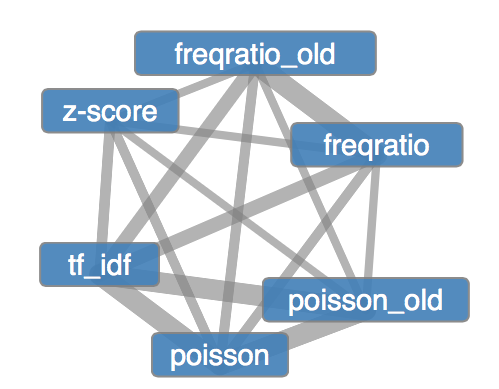
\includegraphics[width=0.7\textwidth]{pictures/comparison.png}
  \caption{Graph of Average Overlap}
  \label{fig:comparisonGraph}
\end{figure}




% SCHLUSS #####################################################################################
\chapter{Bewertung und Zusammenfassung}\label{schluss}
Die Untersuchung der Vergleichsmaße hat das im Projekt \emph{Wörter des Tages} genutzte Poisson Vergleichsmaß als geeignet indentifiziert. Als interessante Verbesserungen wurde die Einbeziehung der Anzahl von Quellen an einem Tag, in denen ein Kandidat auftaucht. Diesen Wert in die Berechnung für ein Maß mit einzubeziehen wurde ausgeschlossen, da bei derzeitigem Datenbankschema die Berechnungzeiten gerade für höherfrequente Worte als zu lang angesehen werden. Das Z-Score Maß liefert auch gute Ergebnisse, allerdings tauchen mehr niederfrequente Worte in der Top-Wort-Liste auf.\\
Die im Abschnitt~\ref{cleaning} aufgeführten regulären Ausdrücke werden als geeignetes Mittel vorgestellt um aktuelle Datumsangaben zu filtern. Eine weitere Methode um strukturbedingt auftauchende Wörter zu filltern liefert die Einbeziehung der oben gennanten Tages-Quellenfrequenz. Tauch ein Wort in den Top-Listen auf, hat aber nur wenige Quellen, weißt das darauf hin, dass es kein Wort ist, welches das tagesaktuelle Geschehen repräsentiert. Viel mehr ist es ein Hinweis auf ein Wort, dass für dass Mass ein außergewöhnliche strukturelle Form widerspiegelt, wie beispielsweise der Name einer interviewten Person, der bei jeder Aussage im Interview wieder genannt wird und deshalb eine hohe Frequenz besitzt.\\
Ein weiteres Mittel um Informationen zu den gefundenen Wörtern aufzubereiten ist der Ansatz der Zeitreihenanalyse, der im Rahmen dieser Arbeit nicht weiter verfolgt werden konnte. Insbesondere zur Visualisierung von Frequenzverläufen einzelner Wörter scheint dies geeignet.\\
Ein weiteres in dieser Arbeit nicht weiter behandeltes Mittel um die Qualität der Ergebnisse zu verbessern ist die Überarbeitung der Liste an genutzten Quellen. Diese, so lassen interessante Wörter wie \emph{Zoo Leipzig} vermuten, haben teils einen regionalen sowie thematischen Schwerpunkt, der bei einer Anzahl von ungefähr 250 Quellen am Tag zu verzerrten Ergebnissen führen kann. Die Auswahl der Quellen scheint für folgende Arbeiten ein interessanter Untersuchungsgegenstand zu sein.



% LITERATUR ####################################################################################
%\nocite{*}%alle nicht aufgeführte Literatur auch auffuehren
\bibliographystyle{plaindin} %alphadin_martin
\bibliography{wortschatzZeitgeistLit} 

\end{document}
